\documentclass[11pt,a4paper]{article}

\usepackage{amsfonts,amssymb,amsmath}
\usepackage[margin=1in]{geometry}
\usepackage[none]{hyphenat}
\usepackage{graphicx}
\usepackage{fancyhdr}
\usepackage{float}
\usepackage{color}
\usepackage{xcolor}
\usepackage{tikz}
\usepackage[nottoc,notlot,notlof]{tocbibind}

\usetikzlibrary{arrows.meta,patterns,shapes}

\parindent 0ex
\setlength{\parskip}{0.55\baselineskip}
\setlength{\abovedisplayskip}{0.5\baselineskip}
\setlength{\belowdisplayskip}{0.5\baselineskip}
\setlength{\abovedisplayshortskip}{0.25\baselineskip}
\setlength{\belowdisplayshortskip}{0.25\baselineskip}
\numberwithin{equation}{section}
% Hyphenation is off, so give TeX a little extra stretch before it settles for an
% overfull line.
\setlength{\emergencystretch}{1.5em}

\pagestyle{fancy}
\fancyfoot[C]{\thepage}
\fancyhead{}
\fancyhead[R]{\rightmark}
\renewcommand{\headrulewidth}{0pt}

% fl(x) is the machine number assigned to x; upright, like any operator.
\DeclareMathOperator{\fl}{fl}
\DeclareMathOperator{\sgn}{sgn}

% Theorem environments.
\usepackage{amsthm}
\theoremstyle{definition}
% One shared counter running section.subsection.n, as in the other courses here.
\newtheorem{thm}{Theorem}[subsection]
\newtheorem{defn}[thm]{Definition}
\newtheorem{exa}[thm]{Example}
\newtheorem{prop}[thm]{Proposition}
\newtheorem{coro}[thm]{Corollary}
\newtheorem{lem}[thm]{Lemma}
\newtheorem{alg}[thm]{Algorithm}
\newtheorem*{note}{Note}
\newtheorem*{remark}{Remark}
\newtheorem{problemx}{Problem}[subsection]
\newenvironment{problem}{\begin{problemx}}{\end{problemx}}
\newenvironment{solution}
  {\renewcommand{\qedsymbol}{}\begin{proof}[\textit{Solution}.]}
  {\end{proof}}
\usepackage{enumitem}
% A heading that is legal inside a theorem body, a list or a float, where
% \subsubsection is not. Same weight as \subsubsection* so the two read alike.
\newcommand{\subhead}[1]{%
  \par\medskip\noindent\textbf{#1}\par\nobreak\smallskip}

\begin{document}
% Title page depersonalised for the web, as with every other course here. The
% formula is the model of floating-point arithmetic on which the error analysis
% of every later section rests.
\begin{titlepage}
\thispagestyle{empty}
\begin{center}
\vspace*{3cm}
{\Huge\bfseries Numerical Methods and Analysis}\\[1.2cm]
{\large Lecture Notes}\\[2.5cm]
\line(1,0){300}\\[1.5cm]
$$\fl(x\odot y) = (x\odot y)(1+\delta),\qquad |\delta|\leq \tfrac{1}{2}\beta^{1-t}$$
\end{center}
\end{titlepage}

\tableofcontents
\thispagestyle{empty}
\clearpage
\setcounter{page}{1}

\section{Mathematical Preliminaries and Error Analysis}
\label{sec:prelim}

Numerical analysis designs methods that produce numbers, and then asks how wrong those numbers can be. Every method in this course
replaces an exact problem (a root, an integral, a solution of a differential equation) by a finite computation, and every computation
is carried out with numbers that have only finitely many digits. So two kinds of error are always present:
\begin{itemize}
\item \textbf{truncation error}, made by the method itself, for example when an infinite series is cut off or a derivative is replaced
by a difference quotient;
\item \textbf{round-off error}, made by the arithmetic, because the computer stores and combines numbers to a fixed number of digits.
\end{itemize}
This section collects the calculus we shall use to bound truncation error, describes how computers represent numbers, and measures the
effect of round-off.

\subsection{Review of calculus}
\label{sec:calc}

The theorems below are proved in a first course in real analysis. They are restated here in the form in which numerical analysis uses
them: each one guarantees that some point exists, and the analysis then uses that point to bound an error.

\begin{thm}[Intermediate Value Theorem]
\label{thm:ivt}
If $f$ is continuous on $[a,b]$ and $K$ is any number between $f(a)$ and $f(b)$, then there is a number $c\in(a,b)$ with $f(c) = K$.
\end{thm}

In particular, if $f(a)$ and $f(b)$ have opposite signs, $f$ has a zero in $(a,b)$. This is the basis of the bisection method in
the next section.

\begin{thm}[Extreme Value Theorem]
\label{thm:evt}
If $f$ is continuous on $[a,b]$, there are points $c_1,c_2\in[a,b]$ with $f(c_1)\leq f(x)\leq f(c_2)$ for all $x\in[a,b]$. If in
addition $f$ is differentiable on $(a,b)$, each of $c_1, c_2$ is either an end point of $[a,b]$ or a point where $f' = 0$.
\end{thm}

The second sentence is how maxima are found in practice: compare the values of $f$ at the end points and at the critical points.

\begin{thm}[Rolle's Theorem and the Mean Value Theorem]
\label{thm:mvt}
Let $f$ be continuous on $[a,b]$ and differentiable on $(a,b)$.
\begin{enumerate}
\item[(a)] If $f(a) = f(b)$, there is $c\in(a,b)$ with $f'(c) = 0$.
\item[(b)] In general there is $c\in(a,b)$ with $f(b) - f(a) = f'(c)(b-a)$.
\end{enumerate}
\end{thm}

\begin{thm}[Generalized Rolle's Theorem]
\label{thm:genrolle}
Let $f\in C[a,b]$ be $n$ times differentiable on $(a,b)$. If $f$ vanishes at $n+1$ distinct points $x_0<x_1<\dots<x_n$ of $[a,b]$, then
$f^{(n)}(c) = 0$ for some $c\in(x_0,x_n)$.
\end{thm}

\begin{proof}
By Rolle's Theorem, $f'$ vanishes at a point of each of the $n$ intervals $(x_{i-1},x_i)$, so $f'$ has $n$ distinct zeros. Applying Rolle's
Theorem to $f'$ between consecutive zeros gives $n-1$ distinct zeros of $f''$, and so on; after $n$ steps $f^{(n)}$ has at least one
zero, lying in $(x_0,x_n)$.
\end{proof}

This theorem is the key to the error formula for polynomial interpolation, later in the course.

\begin{thm}[Weighted Mean Value Theorem for Integrals]
\label{thm:wmvt}
If $f$ is continuous on $[a,b]$, $g$ is integrable on $[a,b]$ and $g$ does not change sign there, then for some $c\in[a,b]$
$$\int_a^b f(x)g(x)\,dx = f(c)\int_a^bg(x)\,dx .$$
\end{thm}

\begin{proof}
Suppose $g\geq0$ (otherwise use $-g$). Let $m$ and $M$ be the minimum and maximum of $f$. Then $mg\leq fg\leq Mg$, and integrating,
$m\int g\leq\int fg\leq M\int g$. If $\int g = 0$ any $c$ works. Otherwise $\int fg/\int g$ lies between $m$ and $M$, and by the
Intermediate Value Theorem it equals $f(c)$ for some $c$.
\end{proof}

This is the tool that turns an error integral into the closed error terms of the quadrature rules for numerical integration.

\begin{thm}[Taylor's Theorem]
\label{thm:taylor}
Suppose $f\in C^n[a,b]$, $f^{(n+1)}$ exists on $[a,b]$, and $x_0\in[a,b]$. Then for every $x\in[a,b]$ there is a number $\xi(x)$ between
$x_0$ and $x$ such that
$$f(x) = P_n(x) + R_n(x),$$
where
\begin{gather*}
P_n(x) = \sum_{k=0}^n\frac{f^{(k)}(x_0)}{k!}(x-x_0)^k ,\\
R_n(x) = \frac{f^{(n+1)}(\xi(x))}{(n+1)!}(x-x_0)^{n+1}.
\end{gather*}
\end{thm}

$P_n$ is the \textbf{$n$th Taylor polynomial} of $f$ about $x_0$ and $R_n$ is the \textbf{remainder} or \textbf{truncation error}. When
$x_0 = 0$ the polynomial is also called a Maclaurin polynomial.

\begin{proof}
Fix $x\neq x_0$ and choose the number $K$ so that
$$f(x) = P_n(x) + K(x-x_0)^{n+1}.$$
Define, for $t$ between $x_0$ and $x$,
$$g(t) = f(x) - \sum_{k=0}^n\frac{f^{(k)}(t)}{k!}(x-t)^k - K(x-t)^{n+1}.$$
Then $g(x) = f(x) - f(x) - 0 = 0$ and $g(x_0) = 0$ by the choice of $K$. By Rolle's Theorem, $g'(\xi) = 0$ for some $\xi$ strictly between
$x_0$ and $x$. Differentiating the sum, the terms telescope:
$$\frac{d}{dt}\sum_{k=0}^n\frac{f^{(k)}(t)}{k!}(x-t)^k = \sum_{k=0}^n\frac{f^{(k+1)}(t)}{k!}(x-t)^k - \sum_{k=1}^n\frac{f^{(k)}(t)}{(k-1)!}(x-t)^{k-1} = \frac{f^{(n+1)}(t)}{n!}(x-t)^n .$$
So
$$0 = g'(\xi) = -\frac{f^{(n+1)}(\xi)}{n!}(x-\xi)^n + (n+1)K(x-\xi)^n ,$$
and since $x-\xi\neq0$, $K = \dfrac{f^{(n+1)}(\xi)}{(n+1)!}$.
\end{proof}

\begin{note}
The point $\xi(x)$ is not known; the theorem only says that it lies between $x_0$ and $x$. Error bounds are obtained by replacing
$|f^{(n+1)}(\xi)|$ by its largest possible value on that interval. This pattern (an exact error formula with an unknown point, followed by
a bound) recurs throughout the course.
\end{note}

\begin{exa}
\label{exa:cos}
Let $f(x) = \cos x$ and $x_0 = 0$.
\begin{enumerate}
\item[(a)] Find the second Taylor polynomial $P_2$ and use it to approximate $\cos 0.01$. Bound the error.
\item[(b)] Use $P_3$ instead and bound the error.
\item[(c)] Use $P_2$ to approximate $\int_0^{0.1}\cos x\,dx$ and bound the error.
\end{enumerate}
\end{exa}

\begin{solution}
The derivatives of $\cos$ at $0$ are $1, 0, -1, 0, 1,\dots$, so
$$\cos x = 1 - \frac{x^2}{2} + \frac{x^3}{6}\sin\xi(x)$$
with $\xi(x)$ between $0$ and $x$.

(a) $P_2(0.01) = 1 - 0.00005 = 0.99995$. The error is $\frac{(0.01)^3}{6}|\sin\xi|$ with $0<\xi<0.01$. Using only $|\sin\xi|\leq 1$
gives the bound $1.\overline{6}\times10^{-7}$. Using $|\sin\xi|\leq|\xi|<0.01$ gives the sharper bound
$$|\cos 0.01 - 0.99995|\leq\frac{(0.01)^3}{6}(0.01)\approx 1.67\times10^{-9}.$$
The actual error is $4.17\times10^{-10}$.

(b) Since the cubic term of the Maclaurin series of $\cos$ is zero, $P_3 = P_2$, but the remainder now has the form
$R_3(x) = \frac{x^4}{24}\cos\xi$, so
$$|\cos0.01 - 0.99995|\leq\frac{(0.01)^4}{24}\approx 4.17\times10^{-10}.$$
The same approximation, analysed with one more term, gets a bound that is almost exactly the true error.

(c) Integrating the identity term by term,
$$\int_0^{0.1}\cos x\,dx = \left[x - \frac{x^3}{6}\right]_0^{0.1} + \int_0^{0.1}\frac{x^3}{6}\sin\xi(x)\,dx = 0.0998\overline{3} + E,$$
with $|E|\leq\int_0^{0.1}\frac{x^3}{6}\,x\,dx = \frac{(0.1)^5}{30}\approx 3.3\times10^{-7}$. In fact $\int_0^{0.1}\cos x\,dx = \sin0.1 =
0.09983341665$, so the error is $8.33\times10^{-8}$.
\end{solution}

\begin{exa}
How many terms of the series $e = \sum_{k=0}^\infty\frac{1}{k!}$ are needed to compute $e$ with an error less than $10^{-6}$?
\end{exa}

\begin{solution}
Taylor's Theorem for $e^x$ about $0$, evaluated at $x=1$, gives
$$e = \sum_{k=0}^n\frac{1}{k!} + \frac{e^{\xi}}{(n+1)!}, \qquad 0<\xi<1.$$
The error is less than $\frac{3}{(n+1)!}$, since $e^\xi<e<3$. We need $(n+1)!>3\times10^6$. Since $9! = 362880$ and $10! = 3628800$,
$n = 9$ suffices: ten terms, $k = 0,\dots,9$, give $e = 2.7182815\ldots$ with error below $8.3\times10^{-7}$.
\end{solution}


\subsection{Round-off errors and computer arithmetic}
\label{sec:fp}

\subhead{Floating-point numbers}
A computer stores a real number in \textbf{floating-point} form
$$\pm\,(0.d_1d_2\ldots d_t)_\beta\times\beta^{e} = \pm\left(\frac{d_1}{\beta}+\frac{d_2}{\beta^2}+\dots+\frac{d_t}{\beta^t}\right)\beta^e,$$
where $\beta$ is the \textbf{base}, $t$ the number of digits of the \textbf{mantissa}, $0\leq d_i\leq\beta-1$, and the \textbf{exponent} $e$
lies in a fixed range $L\leq e\leq U$. The number is \textbf{normalized} if $d_1\neq0$. Only finitely many numbers have this form, and
they are not evenly spaced: between consecutive powers of $\beta$ there are always the same number of them, so the gaps grow with the
size of the numbers.

\begin{figure}[H]
\centering
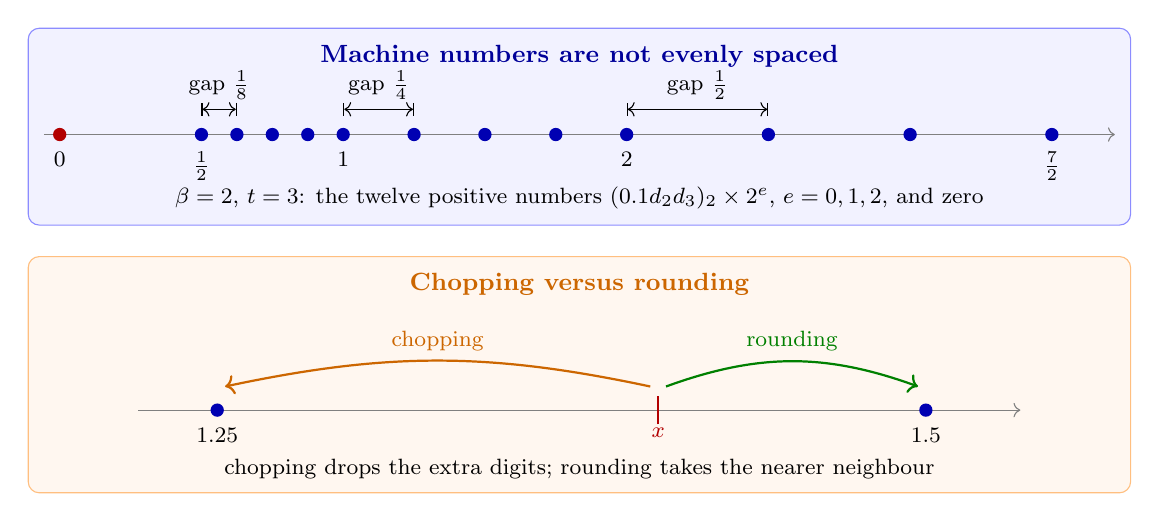
\begin{tikzpicture}
% Panel 1: the toy system beta=2, t=3, e in {0,1,2}; 1 unit of x = 3.6cm
\fill[blue!5,rounded corners] (-0.4,-1.15) rectangle (13.6,1.35);
\draw[blue!45,rounded corners] (-0.4,-1.15) rectangle (13.6,1.35);
\node[font=\small\bfseries,text=blue!60!black] at (6.6,1.0) {Machine numbers are not evenly spaced};
\draw[->,gray] (-0.2,0) -- (13.4,0);
\foreach \x in {0.5,0.625,0.75,0.875,1,1.25,1.5,1.75,2,2.5,3,3.5} \fill[blue!70!black] (\x*3.6,0) circle (2.4pt);
\fill[red!70!black] (0,0) circle (2.4pt);
\foreach \x/\l in {0/0,0.5/{\tfrac12},1/1,2/2,3.5/{\tfrac72}} \node[font=\footnotesize,below] at (\x*3.6,-0.1) {$\l$};
\draw[|<->|,thin] (1.8,0.32) -- node[above,font=\footnotesize]{gap $\tfrac18$} (2.25,0.32);
\draw[|<->|,thin] (3.6,0.32) -- node[above,font=\footnotesize]{gap $\tfrac14$} (4.5,0.32);
\draw[|<->|,thin] (7.2,0.32) -- node[above,font=\footnotesize]{gap $\tfrac12$} (9.0,0.32);
\node[font=\footnotesize] at (6.6,-0.8) {$\beta=2$, $t=3$: the twelve positive numbers $(0.1d_2d_3)_2\times2^e$, $e=0,1,2$, and zero};
% Panel 2: chopping and rounding
\fill[orange!6,rounded corners] (-0.4,-4.55) rectangle (13.6,-1.55);
\draw[orange!50,rounded corners] (-0.4,-4.55) rectangle (13.6,-1.55);
\node[font=\small\bfseries,text=orange!80!black] at (6.6,-1.9) {Chopping versus rounding};
\draw[->,gray] (1,-3.5) -- (12.2,-3.5);
\fill[blue!70!black] (2,-3.5) circle (2.4pt); \fill[blue!70!black] (11,-3.5) circle (2.4pt);
\node[font=\footnotesize,below] at (2,-3.6) {$1.25$};
\node[font=\footnotesize,below] at (11,-3.6) {$1.5$};
\draw[red!70!black,thick] (7.6,-3.68) -- (7.6,-3.32);
\node[font=\footnotesize,red!70!black,below] at (7.6,-3.6) {$x$};
\draw[->,orange!80!black,thick] (7.5,-3.2) to[bend right=12] node[above,font=\footnotesize]{chopping} (2.1,-3.2);
\draw[->,green!50!black,thick] (7.7,-3.2) to[bend left=20] node[above,font=\footnotesize]{rounding} (10.9,-3.2);
\node[font=\footnotesize] at (6.6,-4.25) {chopping drops the extra digits; rounding takes the nearer neighbour};
\end{tikzpicture}
\caption{Top: in a floating-point system the spacing doubles at each power of the base, so the \emph{relative} spacing stays about the
same. Bottom: a real number $x$ between two machine numbers is replaced by the one below it (chopping) or by the nearer one (rounding).}
\label{fig:fpgrid}
\end{figure}

\begin{defn}
The \textbf{IEEE 754 double-precision} format, used by almost all present-day computers, stores a number in 64 bits: one sign bit $s$, an
11-bit exponent $c$ and a 52-bit fraction $f$, representing
$$(-1)^s\,2^{c-1023}\,(1+f), \qquad 0\leq f<1 .$$
The leading $1$ is not stored, so the mantissa effectively has 53 binary digits.
\end{defn}

\begin{exa}
Decode the machine number
$$0\ \ 10000000011\ \ 1011100100010000\ldots0 .$$
\end{exa}

\begin{solution}
The sign bit is $0$, so the number is positive. The exponent is $c = 2^{10}+2^1+2^0 = 1027$, so the power is $2^{1027-1023} = 2^4$. The
fraction is
$$f = \frac12+\frac18+\frac1{16}+\frac1{32}+\frac1{256}+\frac1{4096} = 0.72290039\ldots$$
Hence the number is $2^4(1+f) = 16\times1.722900390625 = 27.56640625$. Its neighbours in the format differ from it by $2^{4-52}\approx
3.6\times10^{-15}$, and every real number within half that distance of it is stored as $27.56640625$.
\end{solution}

\begin{note}
In double precision the largest number is $(2-2^{-52})2^{1023}\approx1.8\times10^{308}$ and the smallest normalized positive number is
$2^{-1022}\approx2.2\times10^{-308}$. Results larger than the first cause \textbf{overflow}; results smaller than the second cause
\textbf{underflow}. The spacing of the numbers next to $1$ is $\varepsilon_{\text{mach}} = 2^{-52}\approx2.22\times10^{-16}$, the
\textbf{machine epsilon}. Double precision therefore carries about $16$ significant decimal digits.
\end{note}

For hand calculation it is convenient to work with $k$-digit decimal numbers $\pm0.d_1d_2\ldots d_k\times10^n$, $d_1\neq0$. Any positive
real number can be written
$$y = 0.d_1d_2\ldots d_kd_{k+1}d_{k+2}\ldots\times10^n .$$
Its floating-point form $\fl(y)$ is obtained by \textbf{chopping}, which simply discards the digits $d_{k+1}d_{k+2}\ldots$, or by
\textbf{rounding}, which adds $5\times10^{n-(k+1)}$ to $y$ and then chops.

\begin{exa}
Give the five-digit chopping and rounding values of $\pi = 0.314159265\ldots\times10^1$.
\end{exa}

\begin{solution}
Chopping: $\fl(\pi) = 0.31415\times10^1 = 3.1415$. Rounding: the sixth digit is $9\geq5$, so the fifth digit is increased:
$\fl(\pi) = 0.31416\times10^1 = 3.1416$.
\end{solution}

\subhead{Measuring error}

\begin{defn}
Let $p^*$ be an approximation to $p$. The \textbf{absolute error} is $|p - p^*|$ and, if $p\neq0$, the \textbf{relative error} is
$\dfrac{|p-p^*|}{|p|}$. The \textbf{percentage error} is $100$ times the relative error.
\end{defn}

\begin{exa}
\label{exa:abserr}
Compare the absolute and relative errors of (a) $p = 0.3000\times10^1$ approximated by $p^* = 0.3100\times10^1$; (b) $p = 0.3000\times
10^{-3}$ by $p^* = 0.3100\times10^{-3}$; (c) $p = 0.3000\times10^4$ by $p^* = 0.3100\times10^4$.
\end{exa}

\begin{solution}
In all three cases the relative error is $\frac{0.0100}{0.3000} = 0.\overline{3}\times10^{-1}$, a percentage error of $3.\overline{3}\%$. The
absolute errors are $0.1$, $0.1\times10^{-4}$ and $0.1\times10^3 = 100$. The absolute error depends on the size of the numbers; the
relative error does not. For this reason the relative error is the better measure of accuracy, and it is the one floating-point
arithmetic controls.
\end{solution}

\begin{defn}
The number $p^*$ approximates $p$ to $t$ \textbf{significant digits} if $t$ is the largest non-negative integer for which
$$\frac{|p-p^*|}{|p|}\leq5\times10^{-t}.$$
\end{defn}

\begin{exa}
How many significant digits do $\frac{22}{7}$, $3.14$ and $3.1416$ give for $\pi$?
\end{exa}

\begin{solution}
The relative errors are
\begin{center}
\begin{tabular}{lcc}
\hline
$p^*$ & relative error & significant digits\\
\hline
$22/7 = 3.142857\ldots$ & $4.02\times10^{-4}$ & $3$\\
$3.14$ & $5.07\times10^{-4}$ & $3$\\
$3.1416$ & $2.34\times10^{-6}$ & $5$\\
\hline
\end{tabular}
\end{center}
For example $4.02\times10^{-4}\leq5\times10^{-3}$ but $4.02\times10^{-4}>5\times10^{-4}$, so $\frac{22}{7}$ gives three significant
digits. The familiar fraction is no better than $3.14$.
\end{solution}

\begin{thm}
\label{thm:fl}
Let $y\neq0$ and let $\fl(y)$ be its $k$-digit decimal floating-point form. Then
$$\frac{|y-\fl(y)|}{|y|}\leq\begin{cases}10^{-k+1}, & \text{chopping},\\[2pt] \tfrac12\times10^{-k+1}, & \text{rounding}.\end{cases}$$
\end{thm}

\begin{proof}
Write $y = 0.d_1d_2\ldots d_kd_{k+1}\ldots\times10^n$ with $d_1\neq0$. For chopping,
$$\frac{|y-\fl(y)|}{|y|} = \frac{0.d_{k+1}d_{k+2}\ldots\times10^{n-k}}{0.d_1d_2\ldots\times10^n} = \frac{0.d_{k+1}d_{k+2}\ldots}{0.d_1d_2\ldots}\times10^{-k}.$$
The numerator is less than $1$ and, since $d_1\geq1$, the denominator is at least $0.1$. So the ratio is at most $\frac{1}{0.1}\times10^{-k}
= 10^{-k+1}$. For rounding, $\fl(y)$ is the nearer of the two $k$-digit neighbours of $y$, which are $10^{n-k}$ apart, so
$|y-\fl(y)|\leq\frac12\times10^{n-k}$, and dividing by $|y|\geq0.1\times10^n$ gives the bound $\frac12\times10^{-k+1}$.
\end{proof}

The number $u = \frac12\beta^{1-t}$ (here $\frac12\times10^{1-k}$) is the \textbf{unit round-off}. The theorem says exactly that
$$\fl(y) = y(1+\delta),\qquad|\delta|\leq u,$$
and computer arithmetic is designed so that the same holds for each operation: if $\odot$ is $+$, $-$, $\times$ or $\div$, then
$\fl(x\odot y) = (x\odot y)(1+\delta)$ with $|\delta|\leq u$. In this model each single operation is accurate; errors arise from
accumulating many operations and, above all, from the next phenomenon.

\subhead{Finite-digit arithmetic and loss of significance}

To model a $k$-digit computer we replace each arithmetic operation by
\begin{align*}
x\oplus y &= \fl(\fl(x)+\fl(y)), & x\ominus y &= \fl(\fl(x)-\fl(y)),\\
x\otimes y &= \fl(\fl(x)\times\fl(y)), & x\oslash y &= \fl(\fl(x)\div\fl(y)).
\end{align*}

\begin{exa}
\label{exa:fivedigit}
Let $x = \frac57$, $y = \frac13$ and $u = 0.714251$, $v = 98765.9$, $w = 0.111111\times10^{-4}$. Use five-digit chopping to compute
$x\oplus y$, $x\ominus u$ and $(x\ominus u)\oslash w$, and find the relative errors.
\end{exa}

\begin{solution}
Here $\fl(x) = 0.71428$, $\fl(y) = 0.33333$ and $\fl(u) = 0.71425$.

$x\oplus y = \fl(1.04761) = 0.10476\times10^1$. The true value is $\frac{22}{21} = 1.047619\ldots$, so the relative error is
$1.8\times10^{-5}$: well within the bound $10^{-4}$ of Theorem~\ref{thm:fl}.

$x\ominus u = 0.71428 - 0.71425 = 0.30000\times10^{-4}$. The true value is $x - u = 0.347143\times10^{-4}$, so the relative error is
$$\frac{0.347143-0.30000}{0.347143} = 0.136 .$$
A single subtraction has produced an answer that is $14\%$ wrong, although both operands were correct to five digits.

$(x\ominus u)\oslash w = \frac{0.30000\times10^{-4}}{0.11111\times10^{-4}} = 0.27000\times10^1$, against the true value $3.1243$: the
large relative error of the difference is carried into the quotient.
\end{solution}

What happened in the subtraction is called \textbf{loss of significance} or \textbf{cancellation}. The leading four digits of
$\fl(x) = 0.71428$ and $\fl(u) = 0.71425$ agree, so they cancel, and the result has only one significant digit: the digit that came from
the rounding errors already present in $x$ and $u$. Subtracting nearly equal numbers does not create error, but it exposes the errors
the numbers already carried, by making them large relative to the answer. Good numerical practice rearranges a calculation to avoid
such subtractions.

\begin{exa}[The quadratic formula]
\label{exa:quadratic}
The roots of $x^2+62.10x+1 = 0$ are $x_1 = -0.01610724$ and $x_2 = -62.08390$, to seven significant digits. Compute them by the
quadratic formula in four-digit rounding arithmetic, and show how to avoid the loss of accuracy.
\end{exa}

\begin{solution}
In four-digit rounding,
$$b^2 - 4ac = 3856 - 4 = 3852,\qquad \sqrt{3852} = 62.06 .$$
The usual formula gives
\begin{gather*}
x_1 = \frac{-62.10+62.06}{2} = \frac{-0.04000}{2} = -0.02000,\\
x_2 = \frac{-62.10-62.06}{2} = -62.08 .
\end{gather*}
The relative error in $x_2$ is $2.6\times10^{-4}$, but in $x_1$ it is
$$\frac{|-0.01611+0.02000|}{0.01611} = 0.24 ,$$
because $-b+\sqrt{b^2-4ac}$ subtracts nearly equal numbers. Rationalizing the numerator removes the subtraction:
$$x_1 = \frac{-b+\sqrt{b^2-4ac}}{2a}\cdot\frac{-b-\sqrt{b^2-4ac}}{-b-\sqrt{b^2-4ac}} = \frac{-2c}{b+\sqrt{b^2-4ac}} = \frac{-2}{62.10+62.06} = \frac{-2}{124.2} = -0.01610,$$
with relative error $4.5\times10^{-4}$. The rule is: when $b>0$ compute $x_2$ from the usual formula and $x_1$ from the rationalized
one (or from $x_1x_2 = c/a$); when $b<0$, do the opposite.
\end{solution}

\begin{exa}[Nested multiplication]
\label{exa:horner}
Evaluate $f(x) = x^3-6.1x^2+3.2x+1.5$ at $x = 4.71$ using three-digit arithmetic, both directly and in the nested form
$f(x) = ((x-6.1)x+3.2)x+1.5$. The exact value is $f(4.71) = -14.263899$.
\end{exa}

\begin{solution}
The intermediate results are:
\begin{center}
\begin{tabular}{lcccccc}
\hline
 & $x^2$ & $x^3$ & $6.1x^2$ & $3.2x$ & direct & nested\\
\hline
chopping & $22.1$ & $104$ & $134$ & $15.0$ & $-13.5$ & $-14.2$\\
rounding & $22.2$ & $105$ & $135$ & $15.1$ & $-13.4$ & $-14.3$\\
\hline
\end{tabular}
\end{center}
With chopping, the direct evaluation has relative error $5.4\%$ and the nested one $0.45\%$; with rounding, $6.1\%$ and $0.25\%$. The
nested form uses two multiplications instead of four, so it is cheaper, and it avoids the subtraction of the large nearly equal numbers
$104$ and $134$. Nested evaluation of polynomials is called \textbf{Horner's method}; we return to it in the section on zeros of polynomials.
\end{solution}


\subsection{Algorithms and convergence}
\label{sec:alg}

An \textbf{algorithm} is a finite sequence of unambiguous steps that produces an approximate solution of a problem. Algorithms in this
course are written in a plain step-by-step form, giving the input, the output and the steps.

Two questions are asked of every algorithm: does the error introduced at one stage grow or die out at later stages, and how fast does
the approximation approach the answer?

\begin{defn}
Suppose an error of size $E_0>0$ is introduced at some stage of a calculation, and $E_n$ denotes its size after $n$ further operations.
If $E_n\approx CnE_0$ for a constant $C$, the growth is \textbf{linear}; if $E_n\approx C^nE_0$ with $C>1$, it is \textbf{exponential}.
An algorithm is \textbf{stable} if small changes in the initial data produce correspondingly small changes in the results, and
\textbf{unstable} otherwise. Linear growth is usually acceptable; exponential growth is not.
\end{defn}

\begin{exa}
\label{exa:recurrence}
For any constants $c_1, c_2$ the sequence $p_n = c_1\left(\frac13\right)^n+c_23^n$ satisfies the recurrence
$$p_n = \tfrac{10}{3}p_{n-1}-p_{n-2},\qquad n = 2,3,\dots$$
With $p_0 = 1$ and $p_1 = \frac13$ the solution is $p_n = \left(\frac13\right)^n$. Compute $p_n$ from the recurrence in five-digit
rounding arithmetic.
\end{exa}

\begin{solution}
That every such $p_n$ satisfies the recurrence is checked by substitution: $\frac{10}3\cdot\frac13 - 1 = \frac19$ and $\frac{10}3\cdot3-1 =
9$, and these are exactly the ratios $\left(\frac13\right)^2$ and $3^2$. The computed values are:
\begin{center}
\begin{tabular}{rlll}
\hline
$n$ & computed $\hat p_n$ & exact $p_n$ & error\\
\hline
$0$ & $1.0000$ & $1.0000$ & $0$\\
$1$ & $0.33333$ & $0.33333\ldots$ & $3.3\times10^{-6}$\\
$2$ & $0.11110$ & $0.11111$ & $1.1\times10^{-5}$\\
$3$ & $0.037000$ & $0.037037$ & $3.7\times10^{-5}$\\
$4$ & $0.012230$ & $0.012346$ & $1.2\times10^{-4}$\\
$5$ & $0.0037660$ & $0.0041152$ & $3.5\times10^{-4}$\\
$6$ & $0.00032300$ & $0.0013717$ & $1.0\times10^{-3}$\\
$7$ & $-0.0026893$ & $0.00045725$ & $3.1\times10^{-3}$\\
$8$ & $-0.0092872$ & $0.00015242$ & $9.4\times10^{-3}$\\
\hline
\end{tabular}
\end{center}
The rounding of $p_1$ (and of $\frac{10}{3}$) means the computation actually follows a solution with a tiny non-zero $c_2$. The term
$c_23^n$ triples at each step, so the error grows exponentially, by a factor of about $3$ per step, and by $n = 7$ the computed values
have the wrong sign. The recurrence is unstable for this problem. By contrast the recurrence $p_n = 2p_{n-1}-p_{n-2}$, whose solutions
$c_1+c_2n$ grow only linearly, started from the same values gives errors that grow only linearly: after eight steps in the same
arithmetic the error is $1.7\times10^{-4}$.
\end{solution}

\subhead{Rates of convergence}

\begin{defn}
Suppose $\beta_n\longrightarrow0$ and $\alpha_n\longrightarrow\alpha$. If there is a constant $K$ such that $|\alpha_n-\alpha|\leq
K|\beta_n|$ for all large $n$, then $\alpha_n$ converges to $\alpha$ with \textbf{rate of convergence} $O(\beta_n)$, and we write
$\alpha_n = \alpha+O(\beta_n)$. Usually $\beta_n = \frac{1}{n^p}$, and we look for the largest $p$.

Similarly, if $G(h)\longrightarrow0$ and $F(h)\longrightarrow L$ as $h\longrightarrow0$, and $|F(h)-L|\leq K|G(h)|$ for all sufficiently
small $h$, we write $F(h) = L+O(G(h))$. Usually $G(h) = h^p$.
\end{defn}

\begin{exa}
Show that $\alpha_n = \frac{n+1}{n^2}$ and $\hat\alpha_n = \frac{n+3}{n^3}$ both converge to $0$, with rates $O\left(\frac1n\right)$ and
$O\left(\frac1{n^2}\right)$.
\end{exa}

\begin{solution}
For $n\geq1$, $\alpha_n = \frac1n+\frac1{n^2}\leq\frac2n$ and $\hat\alpha_n = \frac1{n^2}+\frac3{n^3}\leq\frac4{n^2}$, so $K = 2$ and
$K = 4$ will do. At $n = 100$, $\alpha_n = 0.0101$ and $\hat\alpha_n = 0.000103$: the second sequence is about $100$ times closer to
its limit, as the rates predict.
\end{solution}

\begin{exa}
\label{exa:sinh}
Show that $\dfrac{\sin h}{h} = 1+O(h^2)$ and $\cos h + \frac12h^2 = 1+O(h^4)$ as $h\longrightarrow0$.
\end{exa}

\begin{solution}
By Taylor's Theorem, $\sin h = h - \frac{h^3}{6}+\frac{h^5}{120}\cos\xi$, so
$$\left|\frac{\sin h}{h}-1\right| = \left|-\frac{h^2}{6}+\frac{h^4}{120}\cos\xi\right|\leq\frac{h^2}{6}+\frac{h^4}{120}\leq\frac{h^2}{5}$$
for $|h|\leq1$. Similarly $\cos h = 1-\frac{h^2}{2}+\frac{h^4}{24}\cos\tilde\xi$, so $\left|\cos h+\frac{h^2}{2}-1\right|\leq\frac{h^4}{24}$. Numerically,
$\frac{\sin 0.1}{0.1} = 0.998334$ and $\frac{\sin 0.01}{0.01} = 0.99998333$: reducing $h$ by a factor of $10$ reduces the error by a
factor of $100$, as $O(h^2)$ predicts.
\end{solution}

\begin{defn}
\label{defn:order}
Suppose $p_n\longrightarrow p$ with $p_n\neq p$ for all $n$. If there are constants $\lambda>0$ and $\alpha\geq1$ with
$$\lim_{n\rightarrow\infty}\frac{|p_{n+1}-p|}{|p_n-p|^\alpha} = \lambda,$$
then $\{p_n\}$ converges to $p$ with \textbf{order} $\alpha$ and \textbf{asymptotic error constant} $\lambda$. Order $\alpha = 1$ (with
$\lambda<1$) is \textbf{linear} convergence and $\alpha = 2$ is \textbf{quadratic} convergence.
\end{defn}

\begin{exa}
\label{exa:linquad}
Compare a linearly convergent sequence with $\frac{|p_{n+1}-p|}{|p_n-p|} = 0.5$ and a quadratically convergent sequence with
$\frac{|p_{n+1}-p|}{|p_n-p|^2} = 0.5$, both starting with $|p_0-p| = 1$. How many terms does each need to reach an error of
$10^{-14}$?
\end{exa}

\begin{solution}
For the linear sequence $|p_n-p| = 0.5^n$, which first falls below $10^{-14}$ when $n = 47$. For the quadratic one,
$|p_n-p| = 0.5|p_{n-1}-p|^2$, which gives $|p_n-p| = 0.5^{2^n-1}$:
$$0.5,\quad 0.125,\quad 7.8\times10^{-3},\quad 3.1\times10^{-5},\quad 4.7\times10^{-10},\quad 1.1\times10^{-19},$$
so six steps suffice, against $47$. Quadratic convergence roughly doubles the number of correct digits at each step. This difference is why
Newton's method, which converges quadratically, is so widely used.
\end{solution}


\subsection{Practice Problems}

\begin{problem}
Find the third Taylor polynomial $P_3$ of $f(x) = \ln(1+x)$ about $x_0 = 0$, use it to approximate $\ln 1.1$, and find a bound for the
error. Compare it with the actual error.
\end{problem}
\begin{solution}
$f'(x) = (1+x)^{-1}$, $f''(x) = -(1+x)^{-2}$, $f'''(x) = 2(1+x)^{-3}$, $f^{(4)}(x) = -6(1+x)^{-4}$. So $P_3(x) = x-\frac{x^2}{2}+\frac{x^3}{3}$
and $P_3(0.1) = 0.1-0.005+0.000\overline{3} = 0.095\overline{3}$. The remainder is $R_3(x) = -\frac{6}{(1+\xi)^4}\frac{x^4}{24}$ with
$0<\xi<0.1$, so $|R_3(0.1)|\leq\frac{(0.1)^4}{4} = 2.5\times10^{-5}$. Since $\ln1.1 = 0.0953102$, the actual error is $2.3\times10^{-5}$:
the bound is nearly sharp, because $\xi$ is close to $0$.
\end{solution}

\begin{problem}
Use four-digit rounding arithmetic to compute $\frac{13}{14}-\frac67$ and $\left(\frac{13}{14}-\frac67\right)/(2e-5.4)$, and find the
relative errors.
\end{problem}
\begin{solution}
$\fl\left(\frac{13}{14}\right) = 0.9286$ and $\fl\left(\frac67\right) = 0.8571$, so the difference is $0.07150$; the true value is
$\frac1{14} = 0.0714286$, a relative error of $1.0\times10^{-3}$. For the denominator, $\fl(2e) = \fl(5.43656) = 5.437$ and
$5.437-5.4 = 0.03700$, while the true value is $0.0365637$: relative error $1.2\times10^{-2}$, because the subtraction cancels three
digits. The quotient is $\fl(0.07150/0.03700) = 1.932$, against the true value $1.953540$, a relative error of $1.1\%$. Each subtraction
of nearly equal numbers costs digits.
\end{solution}

\begin{problem}
The function $f(x) = \frac{1-\cos x}{x^2}$ tends to $\frac12$ as $x\longrightarrow0$. Explain why computing it directly for $x = 10^{-5}$
in double precision gives a poor answer, and give an equivalent formula that does not.
\end{problem}
\begin{solution}
For small $x$, $\cos x\approx1-\frac{x^2}{2}$ is very close to $1$, so $1-\cos x$ subtracts nearly equal numbers. At $x = 10^{-5}$,
$1-\cos x\approx5\times10^{-11}$, while the absolute round-off error in $\cos x$ is about $10^{-16}$; the relative error of the difference can therefore be as large as $10^{-16}/(5\times10^{-11}) = 2\times10^{-6}$. In fact double precision
gives $f(10^{-5}) = 0.50000004$, correct to only seven of its sixteen digits, and for $x = 10^{-8}$ it gives $0$, since $\cos x$ rounds
to exactly $1$. Using $1-\cos x = 2\sin^2\frac{x}{2}$,
$$f(x) = \frac{2\sin^2(x/2)}{x^2} = \frac12\left(\frac{\sin(x/2)}{x/2}\right)^2,$$
which involves no subtraction and is accurate for all small $x$.
\end{solution}

\begin{problem}
Show that the $k$-digit rounding of $\frac23$ and of $0.\overline{6}$ are the same, and find the smallest $k$ for which $\fl(\pi)$ (by
rounding) approximates $\pi$ with relative error less than $10^{-6}$.
\end{problem}
\begin{solution}
They are the same number, $0.666\ldots$; its $k$-digit rounding is $0.66\ldots67$ (with $k-1$ sixes). For $\pi$, Theorem~\ref{thm:fl}
guarantees a relative error at most $\frac12\times10^{1-k}$, which is below $10^{-6}$ when $k\geq7$. In fact $k = 6$ already works:
$\fl(\pi) = 3.14159$ has relative error $8.4\times10^{-7}$. The theorem gives a guarantee for every number, not the error for a
particular one.
\end{solution}

\begin{problem}
Show that $\frac{e^h-1}{h} = 1+O(h)$ as $h\longrightarrow0$, and find the rate of convergence of $\frac{e^h-e^{-h}}{2h}$ to $1$.
\end{problem}
\begin{solution}
By Taylor's Theorem $e^h = 1+h+\frac{h^2}{2}e^{\xi}$, so $\frac{e^h-1}{h}-1 = \frac h2e^\xi$, which is at most $\frac{e}{2}|h|$ for $|h|\leq
1$: the rate is $O(h)$. For the symmetric quotient, $e^h-e^{-h} = 2h+\frac{h^3}{3}+\frac{h^5}{60}+\cdots$, so $\frac{e^h-e^{-h}}{2h} =
1+\frac{h^2}{6}+O(h^4)$: the rate is $O(h^2)$. This is the first sign of a fact used in numerical differentiation: a centred difference is
more accurate than a one-sided one.
\end{solution}

\begin{problem}
A sequence satisfies $p_n = p+\frac{1}{n}$. Show that it converges to $p$ sublinearly, that is, $\frac{|p_{n+1}-p|}{|p_n-p|}\longrightarrow
1$, and estimate how many terms are needed for an error below $10^{-6}$. Contrast this with $q_n = p+10^{-n}$.
\end{problem}
\begin{solution}
$\frac{|p_{n+1}-p|}{|p_n-p|} = \frac{n}{n+1}\longrightarrow1$, so the error ratio approaches $1$ and each step gains less and less. An error
below $10^{-6}$ needs $n>10^6$ terms. For $q_n$ the ratio is exactly $\frac{1}{10}$: linear convergence with $\lambda = 0.1$, and seven
terms suffice. Sublinear convergence is far too slow for practical use.
\end{solution}

\clearpage
\section*{References}
\addcontentsline{toc}{section}{References}

\subhead{Prescribed text}
\begin{enumerate}
\item Burden, R. L., and Faires, J. D. (2011), \emph{Numerical Analysis} (9th ed.), Boston, Brooks/Cole, Cengage Learning.
\end{enumerate}

\subhead{Other texts}
\begin{enumerate}
\item Atkinson, K. E. (1989), \emph{An Introduction to Numerical Analysis} (2nd ed.), New York, Wiley.
\item Kincaid, D., and Cheney, W. (2002), \emph{Numerical Analysis: Mathematics of Scientific Computing} (3rd ed.), Pacific Grove, CA,
Brooks/Cole.
\item S\"uli, E., and Mayers, D. F. (2003), \emph{An Introduction to Numerical Analysis}, Cambridge, Cambridge University Press.
\item Higham, N. J. (2002), \emph{Accuracy and Stability of Numerical Algorithms} (2nd ed.), Philadelphia, SIAM.
\end{enumerate}

\subhead{Further reading}
% Long journal names leave no good break point without hyphenation.
\sloppy
\begin{enumerate}
\item Goldberg, D. (1991), What every computer scientist should know about floating-point arithmetic, \emph{ACM Computing Surveys}, 23,
5--48.
\item IEEE (1985), \emph{IEEE Standard for Binary Floating-Point Arithmetic}, ANSI/IEEE Std 754-1985, New York, Institute of Electrical
and Electronics Engineers.
\item Taylor, B. (1715), \emph{Methodus Incrementorum Directa et Inversa}, London.
\item Wilkinson, J. H. (1963), \emph{Rounding Errors in Algebraic Processes}, Englewood Cliffs, NJ, Prentice-Hall.
\end{enumerate}

\end{document}
